\documentclass{article}

\usepackage[utf8]{inputenc}
\usepackage[T1]{fontenc}
\usepackage{lipsum}
\usepackage{graphicx}
\usepackage{amsmath}
\usepackage[margin=1in]{geometry}
\usepackage{titlesec}
\usepackage{enumitem}

\titleformat{\section}
{\LARGE\bfseries}{\thesection}{1em}{}

\titleformat{\subsection}
{\Large\bfseries}{\thesection}{1em}{}

\begin{document}
\pagestyle{empty}
\section*{Diagramma di macchina a stati}
\large
\subsection*{Introduzione}
\large
Obiettivi:
\begin{itemize}[label={-}]
    \itemsep0em
    \item Comprendere il state machine diagram, affinchè possa essere punto di raccordo tra diagramma dei casi d'uso e delle classi
\end{itemize}
UML include la modellazione di \textbf{diagrammi di stato}, principalmente utilizzati per illustrare \textbf{eventi} e \textbf{transizioni}.\ Occorre fin da subito sottolineare la duplice distinzione che contraddistingue questo diagramma, in relazione a due \textbf{modelli comportamentali}, quali:
\begin{itemize}[label={-}]
    \itemsep0em
    \item \textit{Behavioral state machine}, descrive un \textit{evento comportamentale} del sistema o di una parte del sistema, come un \textbf{attraversamento} dei \textit{vertici} che compongono il chart, connessi mediante \textit{transizioni} 
    \item \textit{Protocol state machine}, descrive il ciclo di vita oppure sequenze di interazioni valide per parti del sistema.\ Quindi in questo caso si evince la presenza di un \textit{protocollo}, in grado di poter rescindere quali azioni possano essere considerate corrette o sbagliate
\end{itemize}
Un primo approccio a questa nuova tipologia di chart è dedicata mediante una serie di definizioni informali, che possano garantire una corretta visione di quali strumenti siano necessari pur di poter manipolare questa semantica.

\subsection*{Elementi del diagramma}
\large
Solitamente un \textit{state machine diagram} ritrae tutte le entità che compongono la sintassi del diagramma, illustrando eventi e stati di interesse di un oggetto, narrandone il comportamento dello stesso qualora soggetto a stimoli esterni.\vspace*{14pt}\\
\textit{Definizione informale}\\Un \textbf{evento} è una occorrenza significativa, similmente, anche se ritrae un esempio scontato e banale, può essere (\textit{Alzare la cornetta del telefono}).\vspace*{14pt}\\
\textbf{Trovare qualche nozione al riguardo...}\vspace*{14pt}\\
\textit{Definizione informale}\\Uno \textbf{stato} è la condizione di un oggetto in un dato momento; riprendendo quanto detto prima potrebbe essere indicato uno stato come segue (\textit{Il telefono non termina di squillare fino a quando il ricevitore non alza la cornetta}).\vspace*{14pt}\\
Il concetto su cui si fonda uno \textit{stato} permette di valorizzare il \textit{lifecycle} di un'istanza, come l'esecuzione di un'attività oppure l'attesa posta per la ricezione di un evento specifico.\\
L'uso degli \textit{stati} avviene per differenziare oggetti tra di loro, dove ognuno dei quali assumerà una condizione differente rispetto a stessi dati immessi.\ Quest'ultimo passaggio consente di diversificare due tipologie di stato, quali:
\begin{itemize}[label={-}]
    \itemsep0em
    \item Stato semplice, non ha vertici interni nemmeno transizioni
    \item Stato composto, contiene una o più sottosequenze, o meglio definiti \textit{sottostati}
\end{itemize}
Un'istanza affinchè possa assumere una certa condizione deve essere sottoposta a stimili esterni, i quali comunemente sono denominati \textbf{comportamenti}.\ I \textit{comporamenti} sono artefici del cambiamento di stato di un oggetto, i quali sono riscontrabili in tre differenti fasi, ossia:
\begin{itemize}[label={-}]
    \itemsep0em
    \item \textit{entry}, è comunicativo qualora siano immesse azioni che stimolino lo stato, per cui producendo un risultato osservabile
    \item \textit{exit}, avviene nella fase conclusiva, da cui fuoriesce la transizione necessaria che colleghi uno stato al suo successivo
    \item \textit{doActivity}, è un behavior eseguito assieme ad ulteriori stati associativi, il quale viene interrotto se non conclude la propria esecuzione qualora si esca dallo stato, a causa della transizione 
\end{itemize}
Graficamente uno \textit{stato} è rappresentato mediante un rettangolo con bordi smussati, dove al suo interno possono essere descritti \textit{comportamenti} che si verificano in base allo stato di avanzamento della condizione.\vspace*{14pt}\\
\textit{Definizione informale}\\Una \textbf{transizione} è la relazione tra due \textit{stati}, la quale indica qualora un \textit{evento} si concretizzi, il \textit{token} si muove dallo \textit{stato iniziale}, o meglio antecedente, verso lo \textit{stato successivo}.\ Nuovamente, pur di ottenere un caso reale, si può concludere l'esempio aggiungendo (\textit{Quando l'evento di alzare la cornetta si realizza, il telefono passa dallo stato sonoro allo stato attivo}).\vspace*{14pt}\\
Perciò è definita come il passaggio \textit{atomico} da una \textit{condizione} rispetto alla moltitudine raggiungibile.\ Al di sopra della \textit{transizioni} possono essere poste delle \textbf{guardie}, le quali pongono la possibilità o impossibilità che si concretizzi un evento, contrariamente in assenza, il passaggio dipende unicamente dall'\textit{evento}.\ Una \textit{guardia} è valutata prima che venga completata la \textit{transizione}.\vspace*{7pt}
\begin{center}
    \includegraphics*[width=0.4\textwidth]{foto 1.png}
\end{center}
Rispetto alla notazione introdotta, potrebbero verificarsi casi in cui non sia posta ne una \textit{azione} e nemmeno un \textit{evento}, da cui ne deriva che il passaggio da uno stato precedente ad uno successivo, come potrebbe verificarsi nell'esempio proposto, avvenga senza alcuna interruzione.\vspace*{14pt}\\
\textit{Esempio}
\begin{center}
    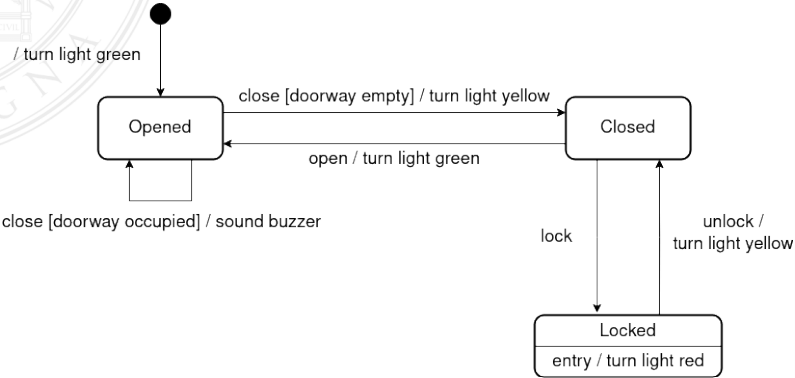
\includegraphics[width=0.66\textwidth]{foto 2.png}
\end{center}
\textit{Nota}: tale modello è usato per esprimere un livello di informazioni piuttosto elevato, molto rigoroso, non contribuendo ad alcuna interpretazione possibile.\vspace*{14pt}\\
Si propone una lettura del diagramma in passaggi consecutivi, che possa anche approcciare a concetti teorici, posta come segue:
\begin{itemize}[label={-}]
    \itemsep0em
    \item Il \textit{nodo totalmente nero} indica il punto di partenza, da cui cominceranno a defluire i differenti token; per certi aspetti simile all'\textit{activity diagram}
    \item Gli stati sono posti dentro rettangoli con bordi smussati.\ \textit{Opened} rappresenta lo stato iniziale, inoltre si ricorda la denominazione data, un participio, il quale indica un atteggiamento passivo rispetto all'azione corrisposta
    \item Le transizioni consistono nei diversi edge, i quali dallo stato iniziale puntano a quello successivo, ma non è escluso che si verifichi esattamente l'opposto.\ Effettività, pur sempre rapportate allo stato \textit{Opened}, sono \textit{close [doorway occupied]}, la quale indica l'impossibilità nell'apertura della porta, quindi conduce nuovamente allo stesso stato trattato e \textit{close [doorway empty]}, ossia è possibile aprire la porta per poi successivamente chiuderla, ponendo l'evento \textit{close} che varierà lo stato a \textit{Closed} 
    \item Ciò che è posto tra le parentesi quadre, come avviene per \textit{[doorway occupied]}, stabiliscono delle \textit{guardie}, le quali operano in maniera piuttosto selettiva; l'impossibilità che un evento non si verifichi è garantita dalla presenza di tale vincolo, la quale pone un giudizio sulla correttezza del passaggio del token
\end{itemize}
Un'ultima considerazione aggiuntiva al diagramma prevede che nessuno stato di per sé abbia comportamenti.\ Uno stato si differenzia da altri corrispettivi poichè prendendo in considerazione \textit{input} differenti corrispondono \textit{output} differenti.
\subsection*{Pseudostati}
\large
\textit{Definizione informale}\\I \textbf{pseudostati} sono elementi sintattici adoperati per arricchire la semantica di un \textit{state machine diagram}.\vspace*{14pt}\\
Ciò che differenzia uno \textit{stato} da un \textit{pseudostato} consiste nel fatto che un \textit{token} di qualsiasi provenienza, non abbia la possibilità di stagnare permanentemente al suo interno.\ Un elemento di questo insieme è \textbf{initial node}, il nodo da cui iniziano a defluire tutti i \textit{marcatori} all'interno della rete.\ Infatti, come da esempio precedente, la \textit{transizione} che collega il \textit{nodo iniziale} allo \textit{stato} successivo non possiede una \textit{guardia}; ciò è regolamentato per ogni \textit{diagram} di tale classe, ovviando ad ogni possibile congettura.\vspace*{14pt}\\
\textit{Initial node} non identifica l'unico pseudostato, ulteriori sono \textbf{join}, \textbf{fork} oppure \textbf{terminate}; quest'ultimo non deve essere confuso con il \textbf{final node}, il proprio obiettivo è totalmente opposto rispetto al secondo citato.\ Spesso il \textit{terminate} è implementato qualora si voglia improntare un particolare \textit{workflow} alla conclusione, senza che risulti essere vincolante per ogni altro token.\vspace*{14pt}\\
Si elencano usi e rappresentazioni grafiche dei pseudostati:
\begin{itemize}[label={-}]
    \itemsep0em
    \item Initial, rappresenta il punto di partenza di una \textit{regione}
    \item Join, simile ad una \textit{swimline} finale, la quale raggruppa differenti transizioni incombi in un'unico edge di uscita.\ Prima di poter uscire al di fuori della \textit{regione}, ogni funzione deve completare le proprie attività
    \item Fork, suddivide una transizione in arrivo in differenti \textit{workflow}.\ Attività contraria rispetto allo \textit{pseudostato join}
    \item ExitPoint, raccordo di conclusione di una \textit{sottomacchina}
    \item Terminate, giunto allo pseudostato l'esecuzione della macchina è conclusa immediatamente
\end{itemize}
\textit{Esempio}\vspace*{7pt}
\begin{center}
    \includegraphics*[width=0.6\textwidth]{foto 3.png}
\end{center}
Un \textit{diagramma di macchina a stati} è adoperato non solo per esprimere nella maniera più dettagliata possibile \textit{eventi} e \textit{transizioni}, ma si presta ottimamente come \textit{design model} per la descrizione di comportamenti per una successiva implementazione.\vspace*{14pt}\\
Per un agevole comprensione è proposto un ulteriore esempio, che raffigura quanto detto prima.\ Posto il \textit{initial node} la fase successiva, la quale comprende una certa \textit{transizione}, è caratterizzata dalla presenza di un'\textit{azione}, in quanto impone il set dei minuti e ore dell'orologio a zero.\vspace*{14pt}\\
Il primo stato analizzato risulta essere \textit{set hours}, il quale pone due tipologie di \textit{behavior} al suo interno: \textit{entry/Beep}, posto per specificare che all'accensione del dispositivo sarà emesso un suono acuto, e \textit{do/Show hours}, quest'ultimo rappresenta un comportamento di lunga durata, ponendo la visualizzazione dell'orario fino a quando non sia stato raggiunto il valore voluto.\vspace*{14pt}\\
Una nota particolare è data dalla presenza di un'\textit{interazione ciclica}, arricchita dall'azione \textit{inc()}, adoperata per poter modificare il valore associativo alle ore dell'orologio; ciò si riscontra esattamente anche nello stato \textit{set minutes}.\ 
Banalmente, i due stati successivi sono perfettamente in linea a quando descritto, ma con alcuni accorgimenti rispetto alla modifica di certi parametri o azioni che debbano conseguire.\vspace*{14pt}\\
Concludendo, l'assenza del \textit{final node} non è un errore, poichè in questo \textit{state machine diagram} i \textit{token} dovranno affluire tra le differenti \textit{transizioni} affinchè sia possibile rispettare la reale volontà nell'uso quotidiano di un orologio.

\subsection*{Regione}
\large 
\textit{Defizione informale}\\Una \textbf{regione} è un insieme di \textit{stati} e \textit{transizioni}, adoperati per rendere maggiormente comprensivo un \textit{diagramma di macchina a stati}.
Spesso la sintassi di una \textit{regione} è utilizzata per manipolare contesti che richiedano un quantitativo di elementi piuttosto articolato e complesso, dove una sua assenza renderebbe di difficile analisi il \textit{diagram} ottenuto.\vspace*{7pt}
\begin{center}
    \includegraphics*[width=0.35\textwidth]{foto 4.png}
\end{center}
Una regione simile, pone una certa effettività.\ Un qualsiasi token che si ritrovi all'interno di uno stato simile provvederà ad affluire nelle due \textbf{submachine} differenti.\ Semplicemente, in questa casistica, le \textit{submachine} definiscono comportamenti interni, destinati a terminare, senza influire su \textit{workflow} esterni.

\subsection*{Sintassi aggiuntiva}
\large
\textit{Definizione informale}\\Una \textbf{compound transitions} rappresenta un insieme di \textit{transizioni} attraversate dal \textit{flow} di \textit{marcatori} generati dal nodo iniziale, le quali non sono vincolate da alcuna \textit{guardia}.\vspace*{14pt}\\
\textit{Esempio}\vspace*{7pt}
\begin{center}
    \includegraphics*[width=0.7\textwidth]{foto 5.png}
\end{center}
Tale \textit{state machine diagram} raffigura una realtà molto particolare, articolata nell'utilizzo di elementi sintattici piuttosto singolari.\vspace*{14pt}\\
E' rappresentato un unico stato, \textit{active}, da cui si diversificano tre \textit{initial dott} differenti.\ Solo una \textit{submachine} è caratterizzata da un \textit{flow} destinato a terminare, ossia la sezione comprendente il concreto lavaggio delle stoviglie.\ La volontà di questa scelta modellativa è dovuta alla continua possibilità, durante l'attivazione della lavastoviglie, di poter modificarne i \textit{pattern} legati alla procedura di lavaggio, come \textit{quick} oppure \textit{normal}.\vspace*{14pt}\\
Si analizza il primo \textit{initial node}.\ Inizializzato il \textit{token}, il primo step consiste nell'acquisizione dello stato \textit{off}, da cui consegue un azione di \textit{setup}, ossia di preparazione al lavaggio.\ Descritto ciò, terminata la fase di preparazione, sono elencati tre \textit{stati successivi}, quali \textit{washing}, \textit{rising} e \textit{drying}.\ La particolarità del \textit{substate} è dovuta all'azione \textit{timeout}; essa, qualora invocata, non provoca una formattazione del processo, ma rimane consistente rispetto all'ultimo stato descrittivo che abbia subito l'azione.\ Quest'ultimo passo è rispecchiato dal termine sintattico \textbf{state history}; mediante tale strumento è possibile tenere traccia dell'attimo in cui si sia verificata un'\textit{interruzione}, garantendo la continuità del \textit{workflow}.\ Contrariamente, pur sempre in relazione ad un \textit{sottostato}, è possibile resettarne il procedimento.\vspace*{14pt}\\
\textit{Esempio}\vspace*{7pt}
\begin{center}
    \includegraphics*[width=0.6\textwidth]{foto 6.png}
\end{center}
\textit{Bank ATM} rappresenta un unica \textit{regione ortogonale}, caratterizzata da un numero piuttosto elevato di \textit{transizioni} tra \textit{stati}.\ Si osserva la presenza di una singola \textit{submachine}, posta all'interno della condizione \textit{Serving Customer}.\vspace*{14pt}\\
Come avviene per il \textit{state diagram Dishwasher}, i \textit{token} inizializzati defluiscono verso lo stato \textit{Off}, per poi convergere verso \textit{Self Test} eseguendo un'azione istantanea di preparazione, denominata \textit{turn on}. Successivamente, attraversando \textit{Idle} e dopo aver inserito la carta di credito, i \textit{marcatori} sono immessi all'interno della sottomacchina. Lo stato in questione permette di prelevare la somma desiderata; certi participi, come \textit{Customer Authentication} e  \textit{Transaction}, possiedono un livello informativo molto più dettagliato, grazie alla presenza di ulteriori \textit{state machine} descrittive, indicate dal simbolo sottostante.\vspace*{14pt}\\
Concludendo, dallo stato \textit{Serving Machine}, scaturiscono tre transizioni, ma ognuna di esse è contraddistinta da un comportamento differente. Nella totalità si analizza un'unica transizione che non abbia un'azione o un evento che la caratterizzi, la quale sarà eseguita senza alcun vincolo; mentre, le due corrispettive, sono adottate qualora l'utente decida di eliminare l'operazione oppure in relazione alla casistica in cui si sia verificato un malfunzionamento provocandone il fallimento, con conseguente inattività della macchina.
\end{document}